\documentclass[conference]{IEEEtran}
\IEEEoverridecommandlockouts
% The preceding line is only needed to identify funding in the first footnote. If that is unneeded, please comment it out.
\usepackage{cite}
\usepackage{amsmath,amssymb,amsfonts}
\usepackage{graphicx}
\usepackage{textcomp}
\usepackage{xcolor}
\def\BibTeX{{\rm B\kern-.05em{\sc i\kern-.025em b}\kern-.08em
    T\kern-.1667em\lower.7ex\hbox{E}\kern-.125emX}}
\begin{document}

\title{CENG435-DATA COMMUNICATIONS AND NETWORKING \\ TERM PROJECT PHASE-1 \\ REPORT \\
{\footnotesize}
\thanks{}
}

\author{\IEEEauthorblockN{ Ahmet Dara VEFA}
\IEEEauthorblockA{\textit{2237899} \\
\textit{Group-68}
}
\and
\IEEEauthorblockN{ Alper KOCAMAN}
\IEEEauthorblockA{\textit{2169589} \\
\textit{Group-68}
}
}

\maketitle

\section{Design and Implementation Part}
\subsection{Project Overview}
This project aims to implement given network topology. This topology comprises a source node, 3 routers namely r1,r2 and r3 and a destination node. UDP(User Datagram Protocol) is used in communication between nodes. Byte streams are sent from source to routers by using this UDP protocol. Router nodes stores the received by stream, sends an acknowledge message to source node and transmit the arrived byte stream to destination node. \\
By using this created network topology, we have done an experiment with different emulation delays. Before doing this experiment, round trip times(RTT) for all  paths between nodes have been calculated in order to use shortest path in the experiment.\\
At the end, by using the results obtained from experiment, we have plotted a network emulation delay vs end to end delay graph. This graph has been plotted with 95\% confidence interval and corresponding standard deviation of the results.\\ 

\subsection{Design Approach}
For RTT part we decided to have a client-server relation between nodes. These relations were(client-server) R1-Source, R1-R2, R1-Destination; R2-Source, R2-Destination; R3-Source, R3-R2, R3-Destination. In order to achieve this, we created one thread for each server and client relation. So R1 created 3 clients, R2 created 2 clients and 2 server, R3 created 3 clients, Source created 3 servers, destination created 3 servers. \\
Clients were used for initiating conversation by sending messages. They would decode and send the current time to the target server by giving Ip version 4(Ipv4) of the link(or interface) and open a port which is used as the address argument. \\
Clients also received replies from the target. These replies were the same as the sent messages. Thus, after decoding the reply, we could obtain the sent time of the message again. This sent time of the message was used to find round trip time of the message. We have subtracted the current time from the reply and we have got the end-to-end delay for the sent message.\\
Servers were used for listening the clients. We have created the server with the Ipv4 address of the link and the port we have chosen to send the messages from the client. We also have given 'names' of the nodes we have been listening for easy identification when saving the average end to end delays between the client and the server.\\
The servers have received data from the clients and have sent the message back if it wasn't empty. We have checked emptiness here since UDP is a protocol which is connectionless and there is no guarantee about message arrival to the destination.\\
The clients would close themselves after sending 1000 messages, receiving the replies and writing the end to end delay to a file. This file was used for calculating statistics about the network delays.Also,the server would close themselves after receiving 1000 messages and sending them back.\\
For the second part, we have used codes similar to part 1. However, this time, there was a change in roles of the nodes. The source would be a client since it was the initiator of the communication. Like source, R3 was also be a client since it has been initiating the communication between destination node. However, since R3 node was a router,  it should listen the source node since it should get the message from source node as well as send the arrival message to the destination. Thus, R3 node was both server and a client. Finally, destination node was a server for R3 since it should listen router 3. \\ 
An acknowledgement system was a requirement in UDP, so we have made that destination and R3 nodes send "ACK" messages to the R3 and Source node respectively. This nodes also have kept sending messages until we received 1000 acknowledgement messages.\\  

\subsection{Implementation Approach}
We chose Python3 as our language since socket programming in it can be done easily. An arbitrary language cannot be selected as implementation language since reserved machines may not have compiler/needed tools for them. Python is a widely used language for socket I/O operations.\\
We have decided to send the current time as the messages since it made it really easy to calculate the delay of the message for us. We have just needed to decode the message and subtract from the current time. \\ 
We chose socket ports from 20445 to 20452 since they were all open. \\
We have built the GENI slice with the given XML on a non-overloaded server since we we didn't want our connection to be laggy.\\
\\
First we wanted to create a connection between source and R1 with our code to test if our client-server code was working. After ensuring our client-server code was working we executed the configure1.sh and conlisten figure2.sh delay scripts. The delays would make create an artificial delay between the nodes, and later we saw this in the average delay reports. \\
The nodes needed to be synchronized their times with the "sudo ntpdate -u pool.ntp.org" command. \\
Then we started executing our python codes. We needed the servers to start before the clients since the clients wouldn't be able to connect or send messages to the server, so we started the servers first, then we started the clients. \\
The clients printed the end to end delay for each message sent to the console. We later copied those values to find the average, standard deviation etc. \\

In order to find the shortest path between source and destination nodes, all paths' value should be found.Our values are:\\
Source-R1:$0.104$\\
Source-R2:$0.143$\\
Source-R3:$0.0004$\\
R1-R2:$0.143$\\
R2-R3:$0.121$\\
R1-Destination:$0.079$\\
R2-Destination:$0.111$\\
R3-Destination:$0.0004$\\

In order to find the shortest path between source node and destination node, we have applied Dijktra's shortest path algorithm. In the first iteration, there is only 1 path is known which is source-source path. The distance of source-source node is naturally 0. Below table shows this situation:(There should be a graph but it's place is shifted due to latex issues)

\begin{table}[h]
\begin{tabular}{|l|l|l|l|l|l|}
\hline
       & SOURCE  & R1 & R2 & R3 & DESTINATION \\ \hline
SOURCE &   0      &  inf  & inf   & inf  & inf       \\ \hline
R1 &    inf     & inf   & inf   & inf   & inf       \\ \hline
R2 &    inf    & inf   &  0  & inf    & inf      \\ \hline
R3 &    inf     & inf   & inf   & inf   &    inf  \\ \hline
DESTINATION &   inf     &  inf  & inf   & inf   & inf     \\ \hline

\end{tabular}
\end{table}

For the second iteration of the algorithm, paths which their distance known are source-R1,source-R2 and source-R3. Below table shows this situation(second table shows):\\ 

\begin{table}[h]
\begin{tabular}{|l|l|l|l|l|l|}
\hline
       & SOURCE  & R1 & R2 & R3 & DESTINATION \\ \hline
SOURCE &   0      &  0.104  & 0.143   &  0.0004  & inf       \\ \hline
R1 &    0.104     & 0   & inf   & inf   & inf       \\ \hline
R2 &    0.143    & inf   &  0  & inf    & inf      \\ \hline
R3 &    0.0004     & inf   & inf   & 0   &    inf  \\ \hline
DESTINATION &   inf     &  inf  & inf   & inf   & 0     \\ \hline

\end{tabular}
\end{table}

Since we don't want to fill our limit with shortest path tables, this is the last table in the shortest path. At the end of iterations, all connected paths distance are known. Since R1 and R3 are not connected, their distance are infinity in the last table.

\begin{table}[h]
\begin{tabular}{|l|l|l|l|l|l|}
\hline
       & SOURCE  & R1 & R2 & R3 & DESTINATION \\ \hline
SOURCE &   0      &  0.104  & 0.143   &  0.0004  & 0.0008   \\ \hline
R1 &    0.104     & 0   & 0.143   & inf   & 0.079   \\ \hline
R2 &    0.143    & 0.143   &  0  & 0.121    & 0.111  \\ \hline
R3 &    0.0004     & inf   & 0.121  & 0   &    0.0004  \\ \hline
DESTINATION &   0.0008 &  0.079  & 0.143   & 0.0004   & 0     \\ \hline

\end{tabular}
\end{table}

It is clearly shown that shortest path between source and destination is Source-R3-Destination way.\\

\section{Methodology and Motivation}
\subsection{Methodology}
We used python's socket library for creating sockets and communicating through them with UDP. \\
We used python's time library for getting time information. \\
We used python's threading library for creating threads for the servers and clients since each server and client ran on different threads. \\

\subsection{Motivation}
We learned the difference between UDP and TCP in this project. Moreover we learned how to use UDP and TCP(even though it was not in the homework) with python. We learnt how to add artificial delays to the links/conncetions.\\
The methods and algorithms we learnt in this homework will be quite useful in our work life since networking is used in almost all sectors of computer engineering.\\

\section{Experimental Results}
\subsection{Used Protocols and Tools For Experiment}
\textbf{Network Time Protocol}:
The first protocol that we have used in order to carry out experiment is NTP(Network Time Protocol).
This protocol is intended to synchronize the computer clocks in a variable-latency, over packet-switched data networks. 

\textbf{Network Emulator}:
NetEm is an abbreviation of NEtwork EMulator. This emulator is emloyed in order to increase the Linux traffic control facilities. With the aid of NetEm, a selected network interface can be calibrated such that delay, packet loss, duplication and more other characteristics can be added to this interface's packets.\\
In the experiment part, this tool is used to emulating the delay on selected interfaces which are source to router 3 interface and router 3 to destination interface. For each interface, 3 different scripts  which have NetEm commands are applied. 

\subsection{Experimental Part}

In the experiment part, we have carried out 3 different experiments. Main task in these experiments were measuring end to end delays between source node and destination node. Between these nodes, router 3 is used which was found the shortest link between them. This end to end delay finding task should be done for 3 different network emulation delays. Thus, we have executed our script for firstly $20ms +-5ms$ normally distributed network emulation delay , afterwards $40ms +-5ms$ normally distributed network emulation delay and finally $50ms +-5ms$ normally distributed network emulation delay. In order to emulate special delays between the nodes, scripts that have NetEm commands are used. One of the script is shown below, this script was used to emulate the interfaces connected to R3 node for $20ms +- 5ms$. \\

\begin{figure}[h]
    \centering
    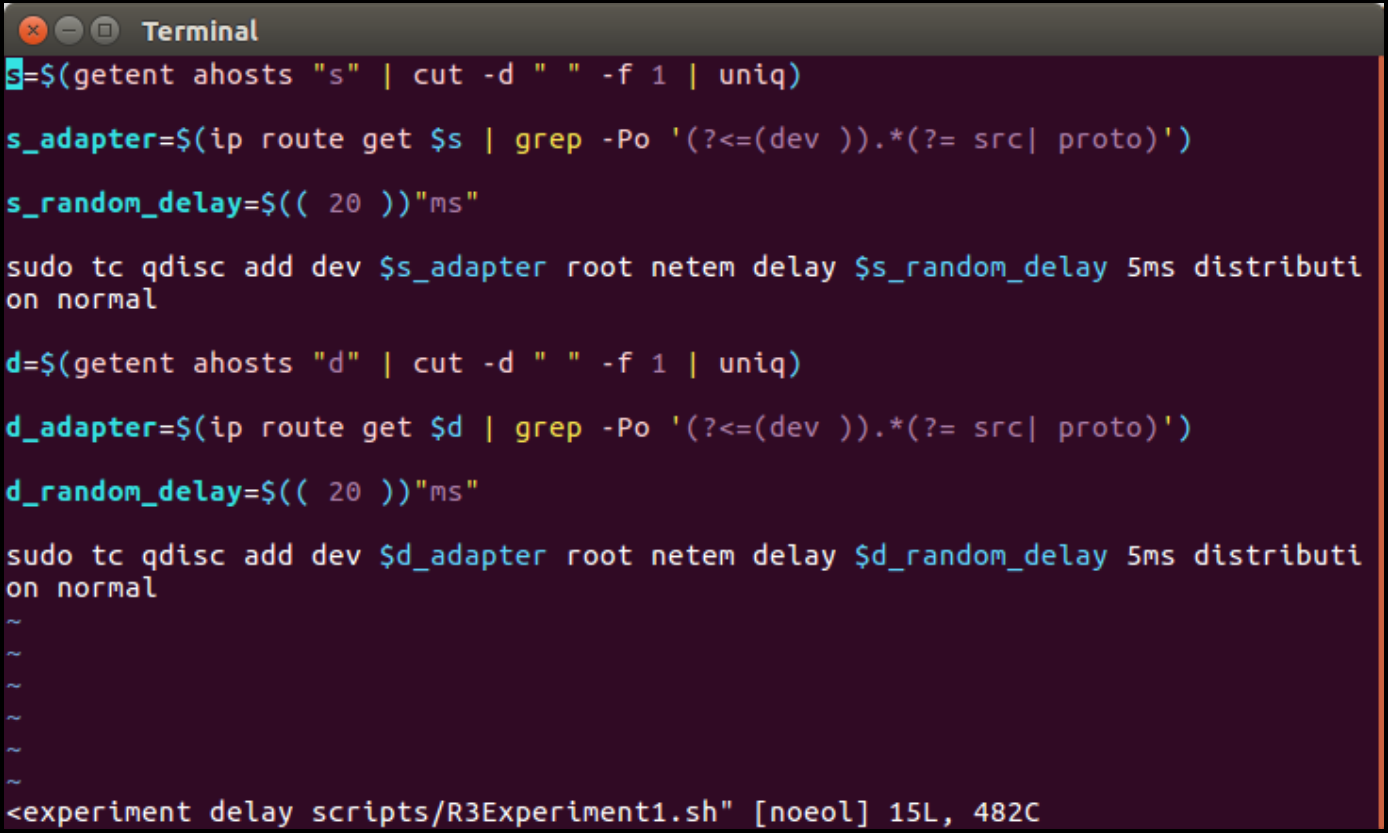
\includegraphics[scale=0.12]{Netem2.png}
    \caption{Example of R3 delay script that has NetEm commands}
\end{figure}

These experiments should be done for noteworthy times in order to get reliable results. Due to this requirement, we have done this experiment for 1000 times for each network emulation delay value. After doing this experiments by 1000 time, we have written output results into a 3 files for each of the network emulation delay. These files contains 1000 delay value for each of the experiments. By looking these values, we collected the required information like standard deviation of the end to end network emulation delays, mean of the end to end network emulation delays etc. Finally, we have plotted the end to end delay vs network emulation delay graph based on our findings. 

\begin{figure}
    \centering
    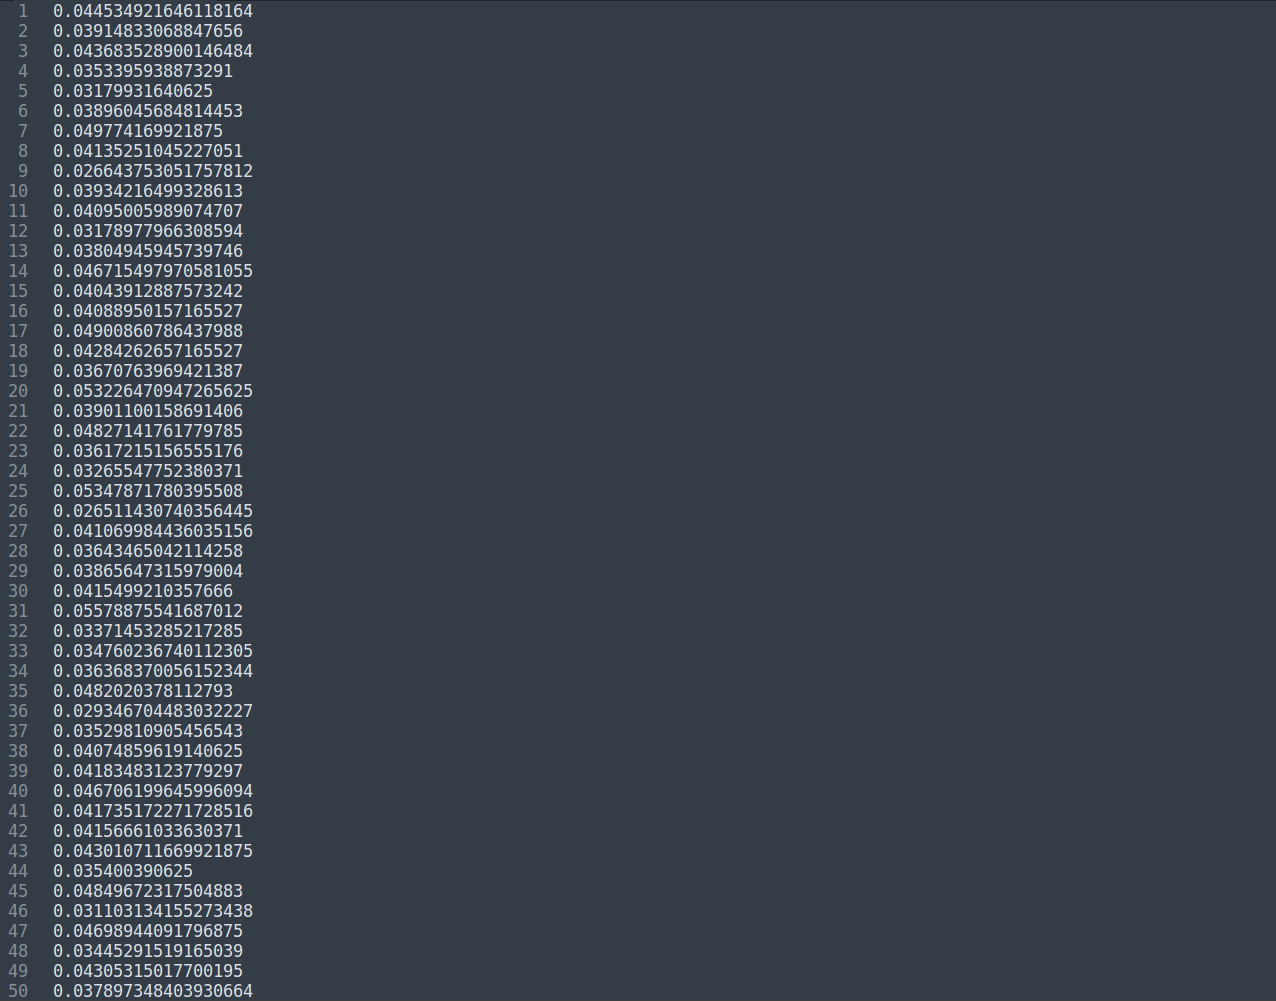
\includegraphics[scale=0.12]{20msresults.png}
    \caption{End-to-End delay result for first 50 packets with network emulation delay $20ms +- 5ms $}
\end{figure}

Error domains for 95\% confidence interval should be obtained in order to plot end to end delay vs network emulation delay. To find these error domains, following formula can be employed for experiments with different network emulation delays: \\

$error = (\text{z value for 95\% confidence interval)} \times \frac{(\text{standard deviation for that experiment's delays})}{\sqrt{\text{number of executions}}} $\\

Since z value is 1.96 for 95\% confidence interval, put these value into the formula,\\

$error = 1.960 \times \frac{(\text{standard deviation for that experiment's delays})}{\sqrt{\text{number of executions}}} $\\

After finding these values, end to end delay gprah can be plotted by using GNU OCTAVE. Following graph shows this plot:\\

Upon calculating these errors, we plotted the end-to-end delay vs network emulation delay graph with the help of Octave. Figure 3 shows this graph clearly. 

\begin{figure}[h]
    \centering
    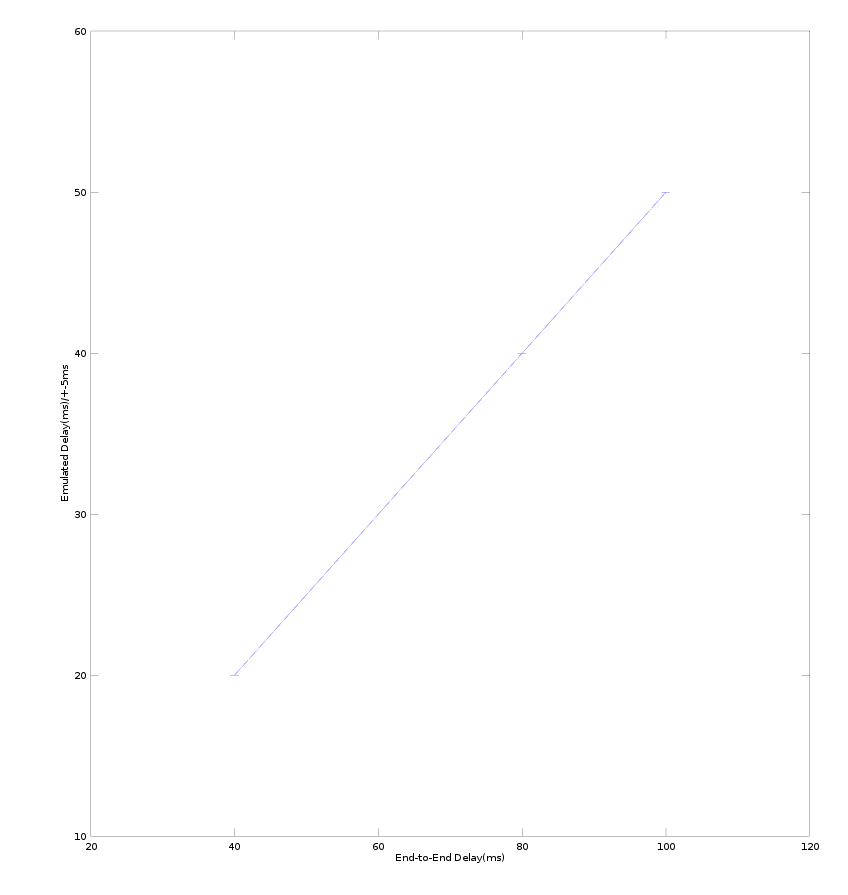
\includegraphics[scale=0.4]{graph.png}
    \caption{Graph of end-to-end delay vs network emulation delay}
\end{figure}


\subsection{Discussion about Experiment Results}
In the experiments,\\
When we apply $20 +-5$ ms normal distributed network emulation delay, average is $0.040575384616852$ seconds = $40$ milliseconds delay and standard deviation is $0.0071340053$.\\

When we apply $40 +-5$ ms normal distributed network emulation delay, average is $0.079376641511917$ seconds  = $80$ milliseconds delay and standard deviation is $0.0071340053$.\\

When we apply $50 +-5$ ms normal distributed network emulation delay, average is $0.099898827314377$ seconds = $100$ milliseconds delay and standard deviation is $0.00714973914$.\\

One of the things should be inferred from the results is when we apply a network emulation delay to a number of links let say n, then there would be an end to end delay which is $n*network\ emulation\ delay\ value$.\\

In our 3 experiments,  we have added a network emulation delay to 2 links which are source-R3 link and R3-destination link. We have expected that these 2 network emulation delays roughly doubles the end to end delay.\\ 
For our first experiment, we have added $20+-5$ ms network emulation delay and get the $40$ ms delay in the average which is 2 times emulated network delay.\\
For our second experiment, we have added $40+-5$ ms network emulation delay and get the $80$ ms delay in the average which is 2 times emulated network delay.\\
For our third experiment, we have added $50+-5$ ms network emulation delay and get the $100$ ms delay in the average which is 2 times emulated network delay.\\


\end{document}